
\breakingframe{
    \begin{textblock*}{13cm}(3.5cm,4cm)
        
    \textbf{\textcolor{black}{Approche bayésienne pour les séries temporelles}}
    \end{textblock*}}

\begin{frame}
    \frametitle{Approche bayésinne pour la modélisation des séries temporelles}
    \setbeamertemplate{itemize items}[triangle]
    \begin{itemize}
        \item Les modèle espace-états      
    \end{itemize}
    \setbeamertemplate{itemize items}[square]
    \bgroup
    \def\arraystretch{1.2}
\begin{table}[]
    \begin{tabular}{lll}
                                                                                               &                                                                         & bruit blanc gaussien       \\ \hline
    \rowcolor[HTML]{96FFFB} 
    \multicolumn{1}{l|}{\cellcolor[HTML]{96FFFB}{\color[HTML]{333333} equation d'observation}} & \multicolumn{1}{l|}{\cellcolor[HTML]{96FFFB}{\color[HTML]{333333} $y_{t} =Z_{t}^{T} \alpha_{t}+\epsilon_{t}$}} & {\color[HTML]{333333} $\epsilon_{t} \sim \mathcal{}{N}\left(0, H_{t}\right)$} \\ \hline
    \rowcolor[HTML]{FFFFC7} 
    \multicolumn{1}{l|}{\cellcolor[HTML]{FFFFC7}{\color[HTML]{333333} equation de transition}} & \multicolumn{1}{l|}{\cellcolor[HTML]{FFFFC7}{\color[HTML]{333333} $\alpha_{t+1} =T_{t} \alpha_{t}+R_{t}\eta_{t} $}} & {\color[HTML]{333333} $ \eta_{t} \sim \mathcal{}{N}\left(0, Q_{t}\right)$} \\
                                                                                               &                                                                         &                           
    \end{tabular}
    \end{table}
    \egroup
    \vspace{-1cm}
        \begin{columns}
        \begin{column}{0.5\textwidth}
            
            \begin{itemize}
                \item $y_t$ observations
                \item $\alpha_t$ variables d'états / latentes / cachées
                \item $Z_t$ matrice de mesure
                \item $T_t$ matrice de transition
            \end{itemize}
        \end{column}
        
        \begin{column}{0.5\textwidth}
            \vspace{0.5cm}
            \begin{figure}
                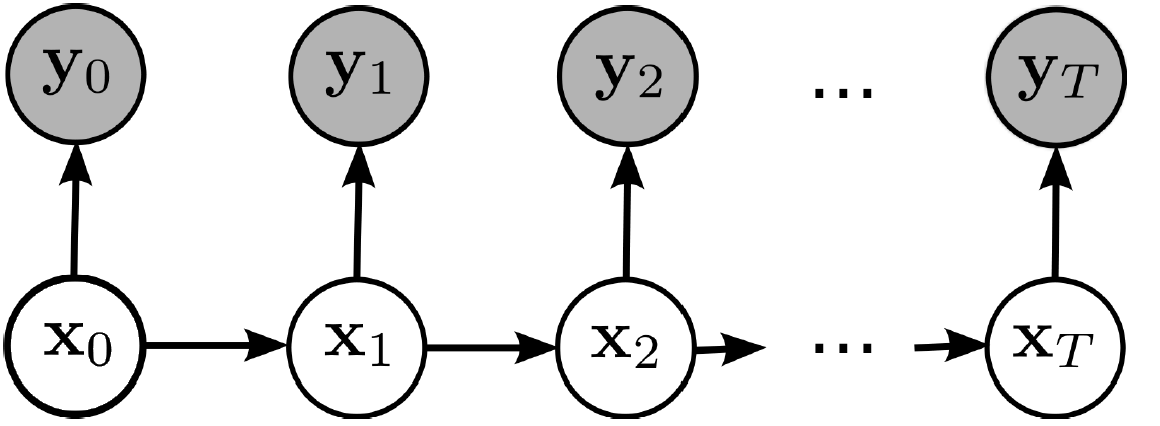
\includegraphics[width=0.8\textwidth]{Figures/hmc.png}
                \caption{Hidden Markov Chain[researchgate.net]}
            \end{figure}
        \end{column}
    \end{columns}
\end{frame}



\begin{frame}
    \frametitle{Approche bayésienne pour la modélisation des séries temporelles}
    
    $\rightarrow$ Bayesian structural time series (BSTS) 
    \bgroup
    \def\arraystretch{1.5}
\begin{table}[]
    \begin{tabular}{lll}
        &                                                                         & bruit blanc gaussien       \\ \hline
\rowcolor[HTML]{96FFFB} 
\multicolumn{1}{l|}{\cellcolor[HTML]{96FFFB}{\color[HTML]{333333} observation}} & \multicolumn{1}{l|}{\cellcolor[HTML]{96FFFB}{\color[HTML]{333333} $y_{t}=\mu_{t}+\beta^{T} x_{t}+\tau_t +\varepsilon_{t}$}}  & {\color[HTML]{333333} $\varepsilon_{t} \sim N\left(0, \sigma_{\varepsilon}^{2}\right)$} \\ \hline
\multicolumn{1}{l|}{regression}                                                 & \multicolumn{1}{l|}{${\beta^{T} x_{t}}$}                                 &                      \\ \hline
\multicolumn{1}{l|}{tendance + marche aléatoire}                                & \multicolumn{1}{l|}{${\mu_{t}=\mu_{t-1}+\delta_{t-1}+u_{t}}$}            & $u_{t} \sim N\left(0, \sigma_{u}^{2}\right)$                        \\ \hline
\multicolumn{1}{l|}{marche aléatoire}                                           & \multicolumn{1}{l|}{$\delta_{t}=\delta_{t-1}+v_{t}$}                     & $v_{t} \sim N\left(0, \sigma_{v}^{2}\right)$                        \\ \hline
\multicolumn{1}{l|}{saisonnalité}                                              & \multicolumn{1}{l|}{$\tau_{t}=-\sum_{s=1}^{s-1} \tau_{t-s}+w_{t}$}       & $w_{t} \sim N\left(0, \sigma_{w}^{2}\right)$                       
\end{tabular}
\end{table}
\egroup
\end{frame}


\begin{frame}
    \frametitle{}
    $\rightarrow$ Bayesian structural time series (BSTS)
    \bgroup
    \def\arraystretch{1.5}
    \begin{table}[]
        \begin{tabular}{l|l|l}
        \rowcolor[HTML]{34CDF9} 
        \multicolumn{1}{l|}{\cellcolor[HTML]{34CDF9}{\color[HTML]{333333} observation}}  & \multicolumn{1}{l|}{\cellcolor[HTML]{34CDF9}{\color[HTML]{333333} $y_{t} =Z_{t}^{T} \alpha_{t}+\epsilon_{t}$}} & {\color[HTML]{333333} $\epsilon_{t} \sim \mathcal{}{N}\left(0, H_{t}\right)$} \\ \hline  
                & \multicolumn{1}{c|}{$Z_t^T$}        & \multicolumn{1}{c|}{$\alpha_t^T$} \\
                    & \multicolumn{1}{c|}{$(\begin{array}{lll}{1} & {0} & {\beta^{T} \mathbf{x}_{t}}\end{array})$}              & \multicolumn{1}{c|}{$\left(\begin{array}{lll}{\mu_{t}} & {\delta_{t}} & {1}\end{array}\right)^{T}$}      \\ \hline
        \rowcolor[HTML]{34CDF9} 
        \multicolumn{1}{l|}{\cellcolor[HTML]{34CDF9}{\color[HTML]{333333} equation de transition}} & \multicolumn{1}{l|}{\cellcolor[HTML]{34CDF9}{\color[HTML]{333333} $\alpha_{t+1} =T_{t} \alpha_{t}+R_{t}\eta_{t} $}} & {\color[HTML]{333333} $ \eta_{t} \sim \mathcal{}{N}\left(0, Q_{t}\right)$} \\
        \multicolumn{1}{c|}{$\alpha_t$}  & \multicolumn{1}{c|}{$T_t$} & \multicolumn{1}{c|}{$N_t \eta_t$}         \\
    \multicolumn{1}{c|}{$\left(\begin{array}{c}{\mu_{t}} \\ {\delta_{t}} \\ {1}\end{array}\right)$}        & \multicolumn{1}{c|}{$\left(\begin{array}{lll}{1} & {1} & {0} \\ {0} & {1} & {0} \\ {0} & {0} & {1}\end{array}\right)$}           & \multicolumn{1}{c|}{$\left(\begin{array}{c}{u_{t}} \\ {v_{t}} \\ {w_t}\end{array}\right)$}       
        \end{tabular}
        \end{table}
        \egroup

        $\rightarrow$ estimation des paramètres
\end{frame}



    




\begin{frame}
    \frametitle{Loi à postériori états cachés $\alpha_t$ : Le filtre de Kalman }
    \centering
    Itérations sur l'estimation $p(\alpha_{t} | y_{1: t}) \sim \mathcal{N}(\hat{\alpha}_{t}, P_t)$
    \begin{figure}
        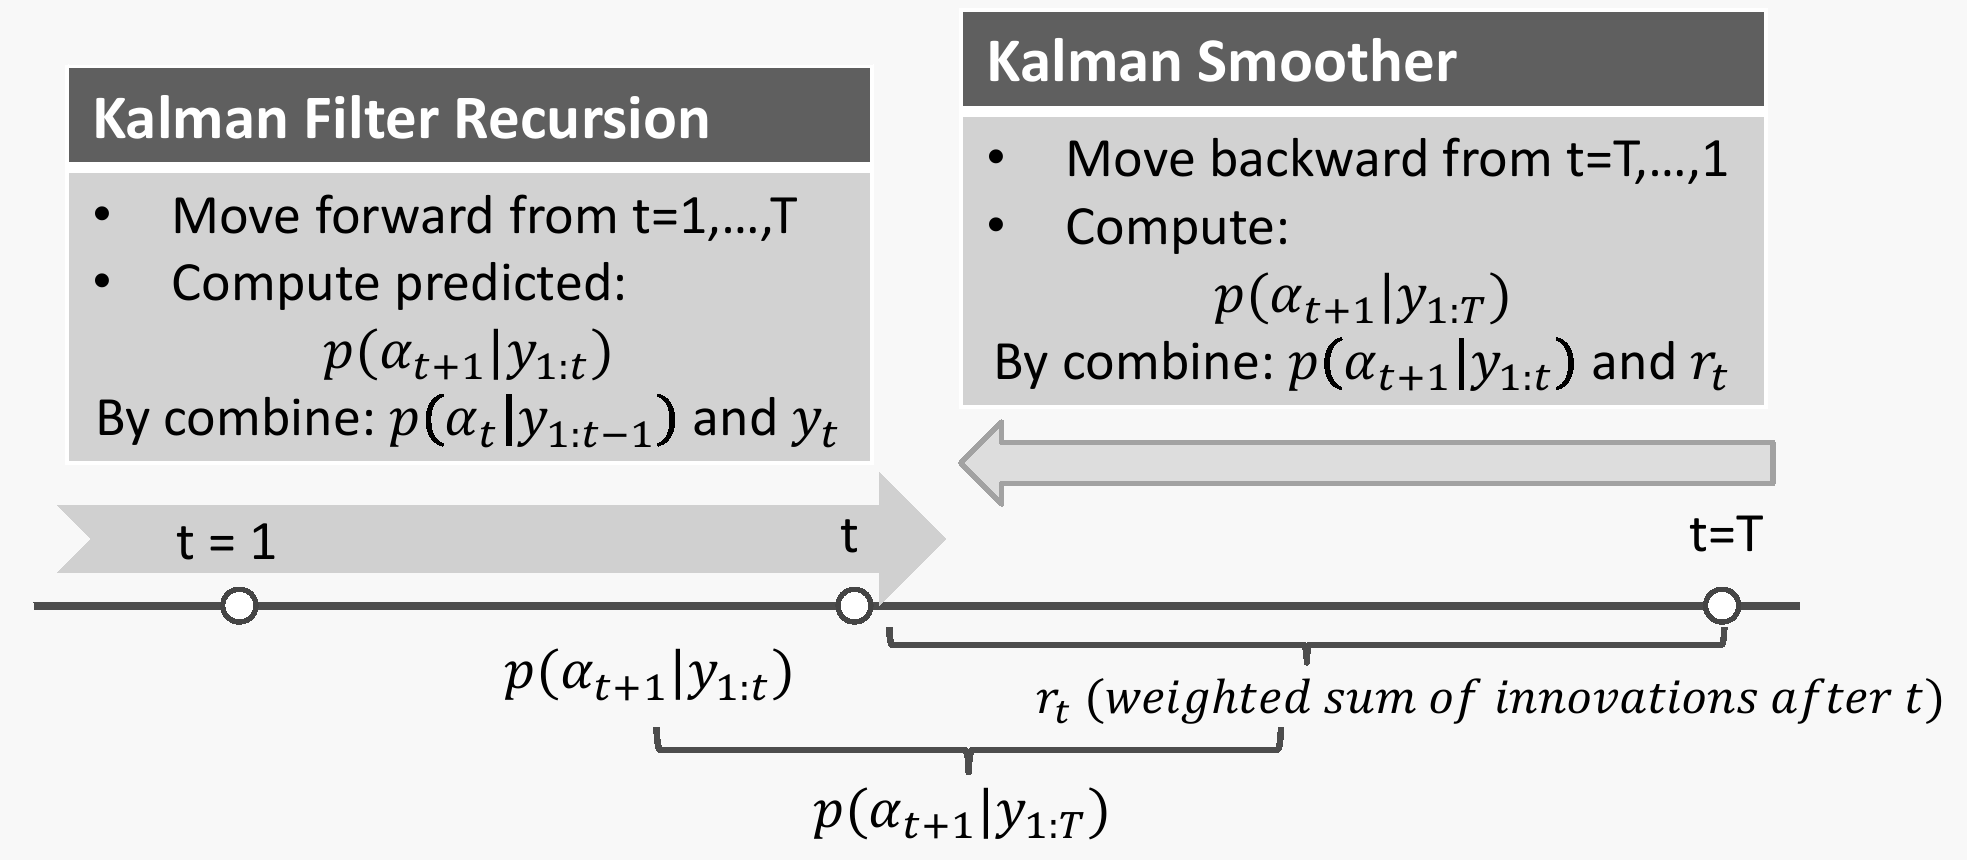
\includegraphics[width=0.8\textwidth]{Figures/kalman_filter.png}
        \caption{[github : anhdanggit/nowcasting-google-queries/]}
    \end{figure}
    
    
\end{frame}

\begin{frame}
    \frametitle{Loi à postériori de $\beta$: \textit{spike-and-slab prior}}
    \vspace{-1cm}
    \begin{columns}
        \begin{column}{0.8\textwidth}
            \vspace{-1cm}
            \begin{itemize}
                \item On prend la partie regression $y_{t}^{*}=y_{t}-\mu_{t}$
                \item On utilise pour $\beta$ une distribution à priori \textit{spike-and-slab}:
            \end{itemize}
            
        \end{column}
        \begin{column}{0.2\textwidth}

            \begin{figure}
                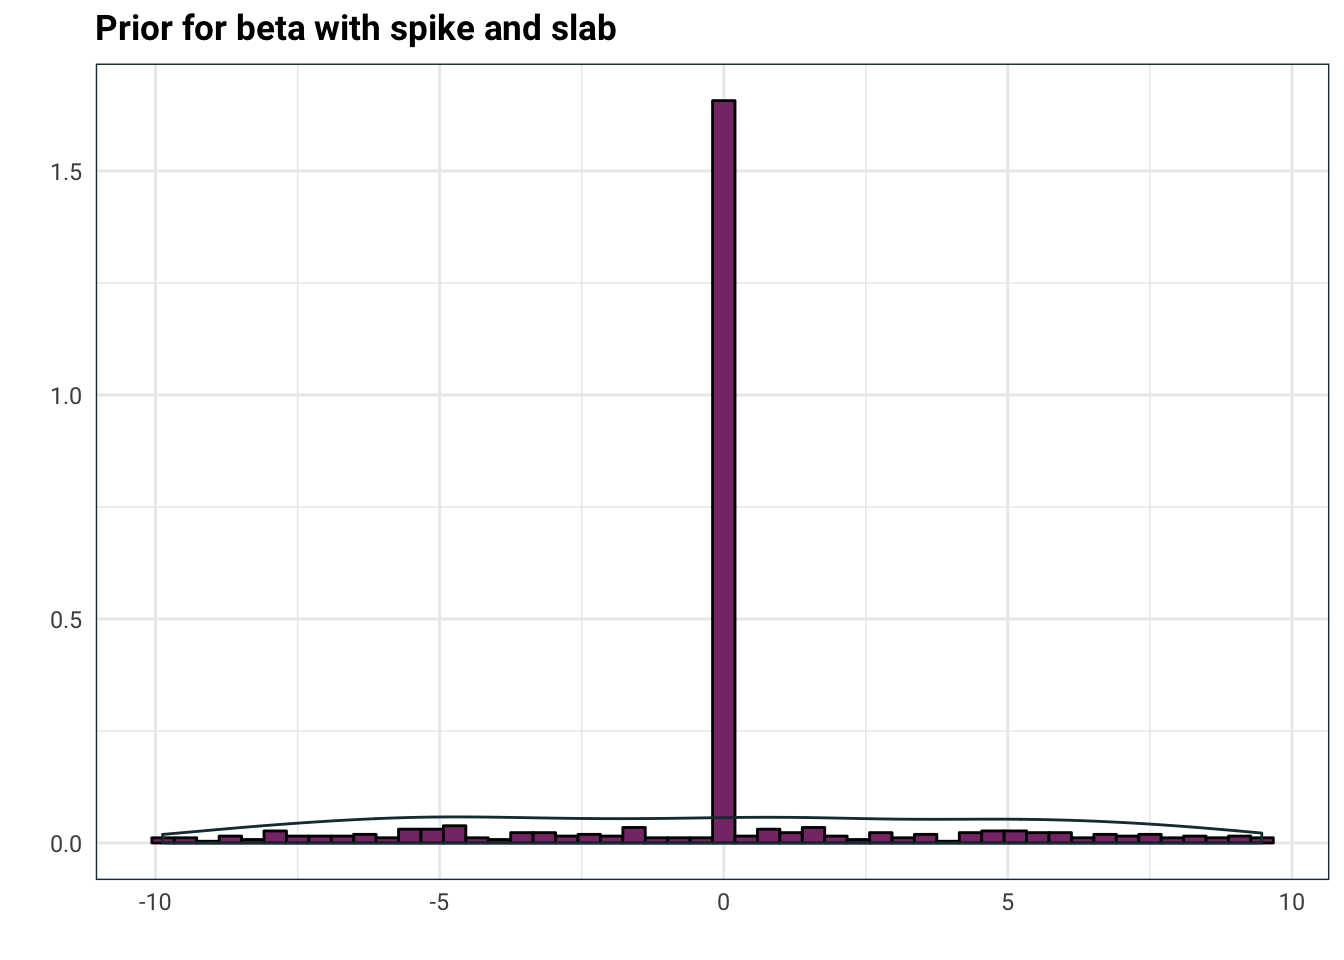
\includegraphics[width=\textwidth]{Figures/pike.png}
                \caption{[batisengul.co.uk]}
            \end{figure}
        
        \end{column}
\end{columns}
\vspace{-1.5cm}
       \setbeamertemplate{itemize items}[triangle]
     
           
    
        \begin{itemize}
            \item  $\displaystyle p(\gamma)=\prod_{k=1}^{N} \pi^{\gamma_k}(1-\pi)^{1-\gamma_k}$, $\gamma_k \in \{0,1 \}$ {\small $N = Card(\mathbf{x})$} 
            \item \'A priori : $p\left(\beta, \gamma, \sigma_{\varepsilon}^{2}\right)=p\left(\beta_{\gamma} | \gamma, \sigma_{\varepsilon}^{2}\right) p\left(\sigma_{\varepsilon}^{2} | \gamma\right) p(\gamma)$ 
            \hfill $\beta_{\gamma} = \beta[\gamma_k \neq 0]$
            \item $
                \beta_{\gamma}\left|\sigma_{\epsilon}^{2}, \gamma \sim \mathcal{N}\left(b_{\gamma},
                \sigma_{\epsilon}^{2}\left(\Omega_{\gamma}^{-1}\right)^{-1}\right) \quad \sigma_{\epsilon}^{2}\right| \gamma \sim IG\left(\frac{\nu}{2}, \frac{s s}{2}\right)
                $ \\ \vspace{0.2cm}
                {\centering \tiny
                papramètres à priori : $v$ nombre de paramètres,$\quad$ $\frac{s s}{v}=\left(1-R^{2}\right) s_{y}^{2}$, $\quad$         $\Omega^{-1} \propto X^{T} X$ }
        \end{itemize}
    
        \setbeamertemplate{itemize items}[square]
   
    \begin{itemize}
        
        \item On utilise les propriété des lois conjugé pour obtenir les loi à postériori \\ \vspace{0.1cm}
        {\centering
        $\beta_{\gamma} | \sigma_{\epsilon}, \gamma, \mathbf{y}^{*} \quad \quad \gamma_\epsilon^{2} | \gamma, \mathbf{y}^{*} \quad \quad \gamma | \mathbf{y}^{*}$}
        \item Intérêt de la \textit{spike-and-slab}
    \end{itemize}

\end{frame}

\begin{frame}
    \small
\begin{exampleblock}{\'Echantilloneur de Gibbs pour BSTS : SSVS algorithm}
    \setbeamertemplate{itemize items}[triangle]
    $\Theta=\left(\gamma, \beta, \sigma_{\varepsilon}^{2}, \sigma_{v}^{2}, \sigma_{u}^{2}\right)$
    \begin{itemize}
    \item Choisir paramètres à priori $v$, $R^2$, $s_y^2$, $\pi$ 
    \item Tirer $\gamma, \beta, \sigma_{\varepsilon}^{2}, \sigma_{v}^{2}, \sigma_{u}^{2}$ \hfill $\sigma_u^2$,$\sigma_u^2$,$\sigma_w^2$ sont tiré selon la loi $. | \gamma \sim I G\left(\frac{\nu}{2}, \frac{s s}{2}\right)$
    \end{itemize}
Sur $1, \ldots, M$:
\begin{enumerate}
\item Après application du filtre de Kalman, on tire les états latents $\alpha$ depuis $p\left(\alpha | y, \gamma, \beta, \sigma_{\varepsilon}^{2}, \sigma_{v}^{2}, \sigma_{u}^{2}\right)$
\item On tire $\sigma_u^2$ et $\sigma_v^2$ selon $p\left(\frac{1}{\sigma_{u}^{2}}, \frac{1}{\sigma_{v}^{2}} | y, \alpha, \beta, \sigma_{\varepsilon}^{2}\right)$
\item On tire $\beta$ et $\sigma_\epsilon^2$ selon $p\left(\beta, \sigma_{\varepsilon}^{2} | y, \alpha, \sigma_{u}^{2}, \sigma_{v}^{2}\right)$
\end{enumerate}

On prend comme modèle la moyenne des tirages $\left(\Theta^m, \ldots, \Theta^M\right)$

\end{exampleblock}

\end{frame}
